%%%%%%%%%%%%%%%%%%%%%%%%%%%%%%%%%%%%%%%%%%%%%%%%%%%%%%%%%%%%%%%%%%%%%%%%%%%%%%%%%%%%%%%%%%%%%%%%
%
% CS484 Written Question Template
%
% Acknowledgements:
% The original code is written by Prof. James Tompkin (james_tompkin@brown.edu).
% The second version is revised by Prof. Min H. Kim (minhkim@kaist.ac.kr).
%
% This is a LaTeX document. LaTeX is a markup language for producing 
% documents. Your task is to fill out this document, then to compile 
% it into a PDF document. 
%
% 
% TO COMPILE:
% > pdflatex thisfile.tex
%
% If you do not have LaTeX and need a LaTeX distribution:
% - Personal laptops (all common OS): www.latex-project.org/get/
% - We recommend latex compiler miktex (https://miktex.org/) for windows,
%   macTex (http://www.tug.org/mactex/) for macOS users.
%   And TeXstudio(http://www.texstudio.org/) for latex editor.
%   You should install both compiler and editor for editing latex.
%   The another option is Overleaf (https://www.overleaf.com/) which is 
%   an online latex editor.
%
% If you need help with LaTeX, please come to office hours. 
% Or, there is plenty of help online:
% https://en.wikibooks.org/wiki/LaTeX
%
% Good luck!
% Min and the CS484 staff
%
%%%%%%%%%%%%%%%%%%%%%%%%%%%%%%%%%%%%%%%%%%%%%%%%%%%%%%%%%%%%%%%%%%%%%%%%%%%%%%%%%%%%%%%%%%%%%%%%
%
% How to include two graphics on the same line:
% 
% \includegraphics[width=0.49\linewidth]{yourgraphic1.png}
% \includegraphics[width=0.49\linewidth]{yourgraphic2.png}
%
% How to include equations:
%
% \begin{equation}
% y = mx+c
% \end{equation}
% 
%%%%%%%%%%%%%%%%%%%%%%%%%%%%%%%%%%%%%%%%%%%%%%%%%%%%%%%%%%%%%%%%%%%%%%%%%%%%%%%%%%%%%%%%%%%%%%%%

\documentclass[11pt]{article}

\usepackage[english]{babel}
\usepackage[utf8]{inputenc}
\usepackage[colorlinks = true,
            linkcolor = blue,
            urlcolor  = blue]{hyperref}
\usepackage[a4paper,margin=1.5in]{geometry}
\usepackage{stackengine,graphicx}
\usepackage{fancyhdr}
\setlength{\headheight}{15pt}
\usepackage{microtype}
\usepackage{times}
\usepackage{booktabs}

% From https://ctan.org/pkg/matlab-prettifier
\usepackage[numbered,framed]{matlab-prettifier}

\frenchspacing
\setlength{\parindent}{0cm} % Default is 15pt.
\setlength{\parskip}{0.3cm plus1mm minus1mm}

\pagestyle{fancy}
\fancyhf{}
\lhead{Homework Writeup}
\rhead{CS484}
\rfoot{\thepage}

\date{}

\title{\vspace{-1cm}Homework 3 Writeup}


\begin{document}
\maketitle
\vspace{-3cm}
\thispagestyle{fancy}

\section*{Instructions}
\begin{itemize}
  \item Describe any interesting decisions you made to write your algorithm.
  \item Show and discuss the results of your algorithm.
  \item Feel free to include code snippets, images, and equations.
  \item Use as many pages as you need, but err on the short side If you feel you only need to write a short amount to meet the brief, th
  
  \item \textbf{Please make this document anonymous.}
\end{itemize}

\section*{In the beginning...}

Harris corner detection and SIFT method is famous method for finding and matching the corners in two different images, has some same content in it.
In this project, I have implemented Harris corner detector to find interesting points. Then implemented some SIFT-like to get the orientation for each windows and made histogram.
Finally, I had to implement feature matching algorithm, by calculating euclidean distance and extract nearest neighbors' ratios.

\section*{Interesting Implementation Detail}

\begin{lstlisting}[style=Matlab-editor]
localmaxima_C = zeros(size(C));
WINSIZE = 2;

for i = 1 + WINSIZE : size(C, 1) - WINSIZE
    for j = 1 + WINSIZE : size(C, 2) - WINSIZE
        tmp_window = C(i - WINSIZE : i + WINSIZE, j - WINSIZE : j + WINSIZE);
        local_maxima = max(tmp_window(:));
        if C(i, j) == local_maxima
            localmaxima_C(i, j) = C(i, j);
        end
    end
end
\end{lstlisting}

I have implemented my own non-maximum suppression algorithm. After calculated C, this algorithm take a look at neighbor values for every values.
``Neighbor values'' are defined by the constant WINSIZE. If the value is local maximum, we keep it. If it's not, it will be 0.

\begin{lstlisting}[style=Matlab-editor]
for fx = 1:4
    for fy = 1:4
        tmp_hist = zeros(1, 8);
        
        for wx = 1:4
            for wy = 1:4
                curr_x = (fx - 1) * 4 + wx;
                curr_y = (fy - 1) * 4 + wy;

                curr_dir = frame_dir(curr_x, curr_y);
                idx = floor(mod(curr_dir + 180, 360) / 45) + 1;
                tmp_hist(idx) = tmp_hist(idx) + frame_mag(curr_x, curr_y);
            end
        end

        idx = (fx - 1) * 32 + (fy - 1) * 8 + 1;
        features(i, idx : idx + 7) = tmp_hist;
    end
end

features(i, :) = features(i, :) / norm(features(i, :));
\end{lstlisting}

I made a histogram for every frames, composed by 4x4 windows. In histogram, [-180, -135) degrees will be the index 1 in histogram, [-135, -90) will be 2, ....
Every histogram calculated from each windows would be a part of the feature.

\vspace{1cm}

\begin{lstlisting}[style=Matlab-editor]
[n1, f] = size(features1);
[n2, f] = size(features2);

dists = zeros(n1, n2);
for i = 1 : n1
    for j = 1 : n2
        dists(i, j) = norm(features1(i, :) - features2(j, :));
    end
end
\end{lstlisting}
norm function in the MATLAB was useful to calculate the euclidean distance.

\pagebreak

\section*{A Result}

\begin{table}[!htbp]
    \centering
    \begin{tabular}{c | cc}
     Sample & Accuracy(All) & Accuracy(100)  \\ \hline
     Notre Dame de Paris &  57.92\% & 90\% \\
     Mountain Rushmore & 63.18\% & 97\%  \\
     Gaudi's Episcopal Palace & 6.667\% & 7\% \\
    \end{tabular}
\end{table}

\begin{figure}[h]
    \centering
    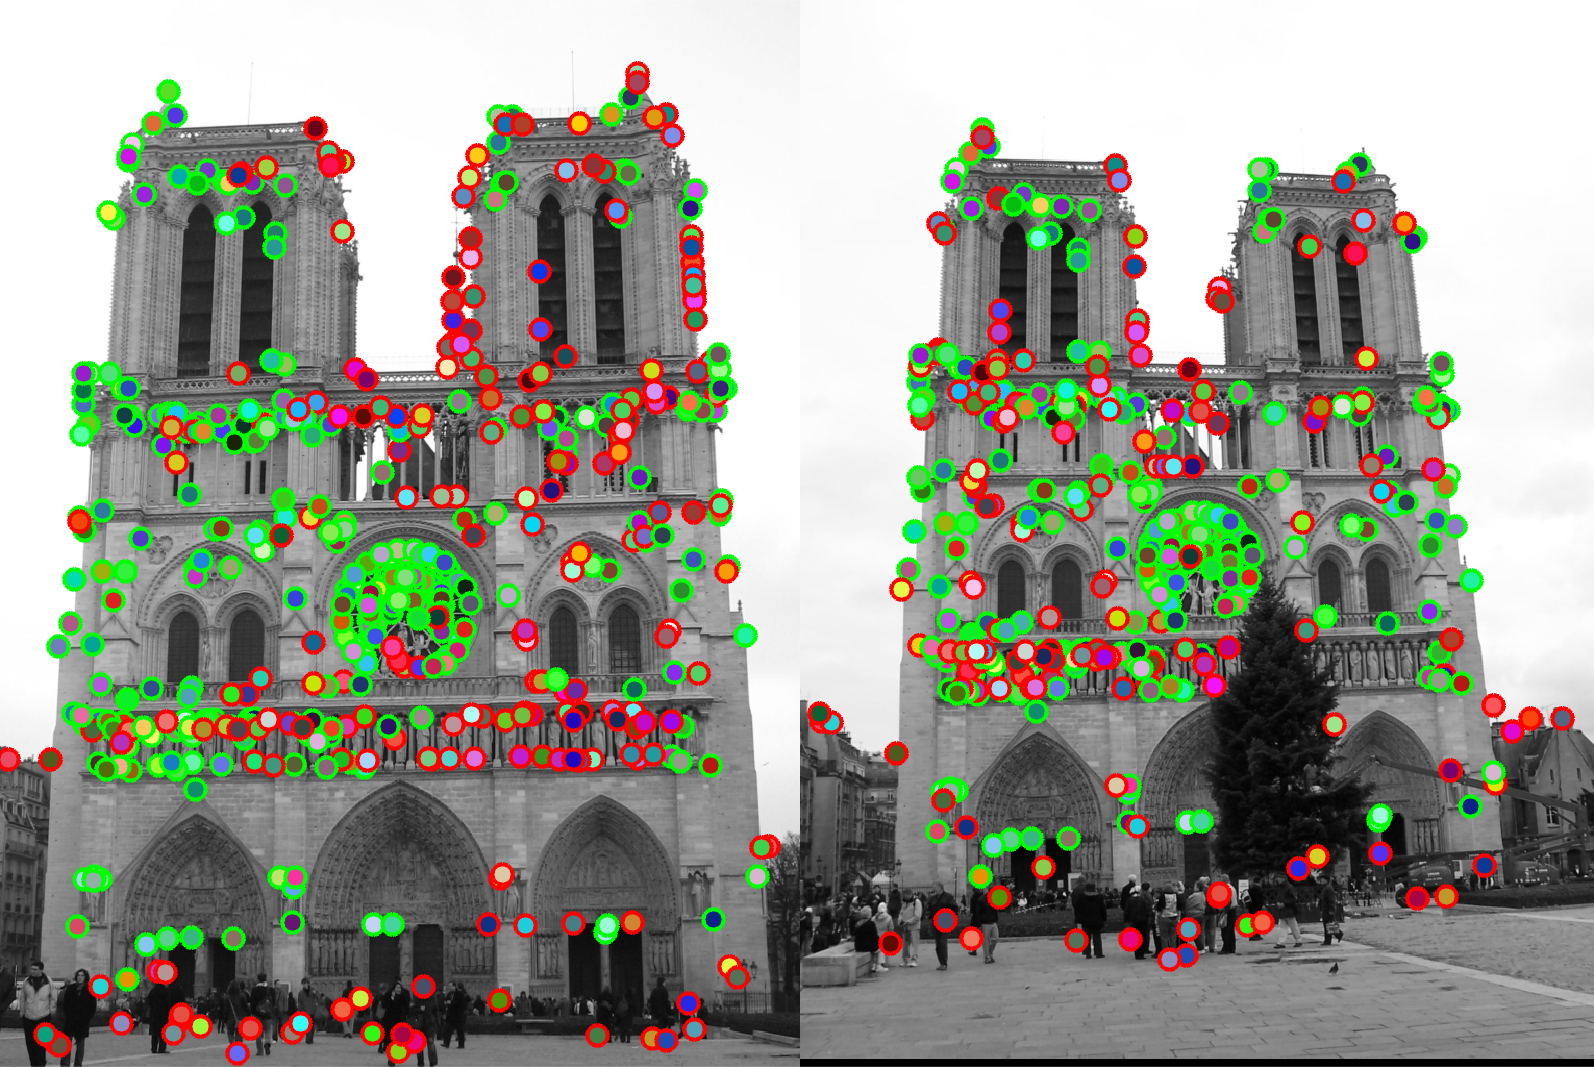
\includegraphics[width=12cm]{../code/eval_ND.png}
    \caption{Result of Notre Dame de Paris}
    \label{fig:Notre Dame de Paris}
\end{figure}

\begin{figure}[h]
    \centering
    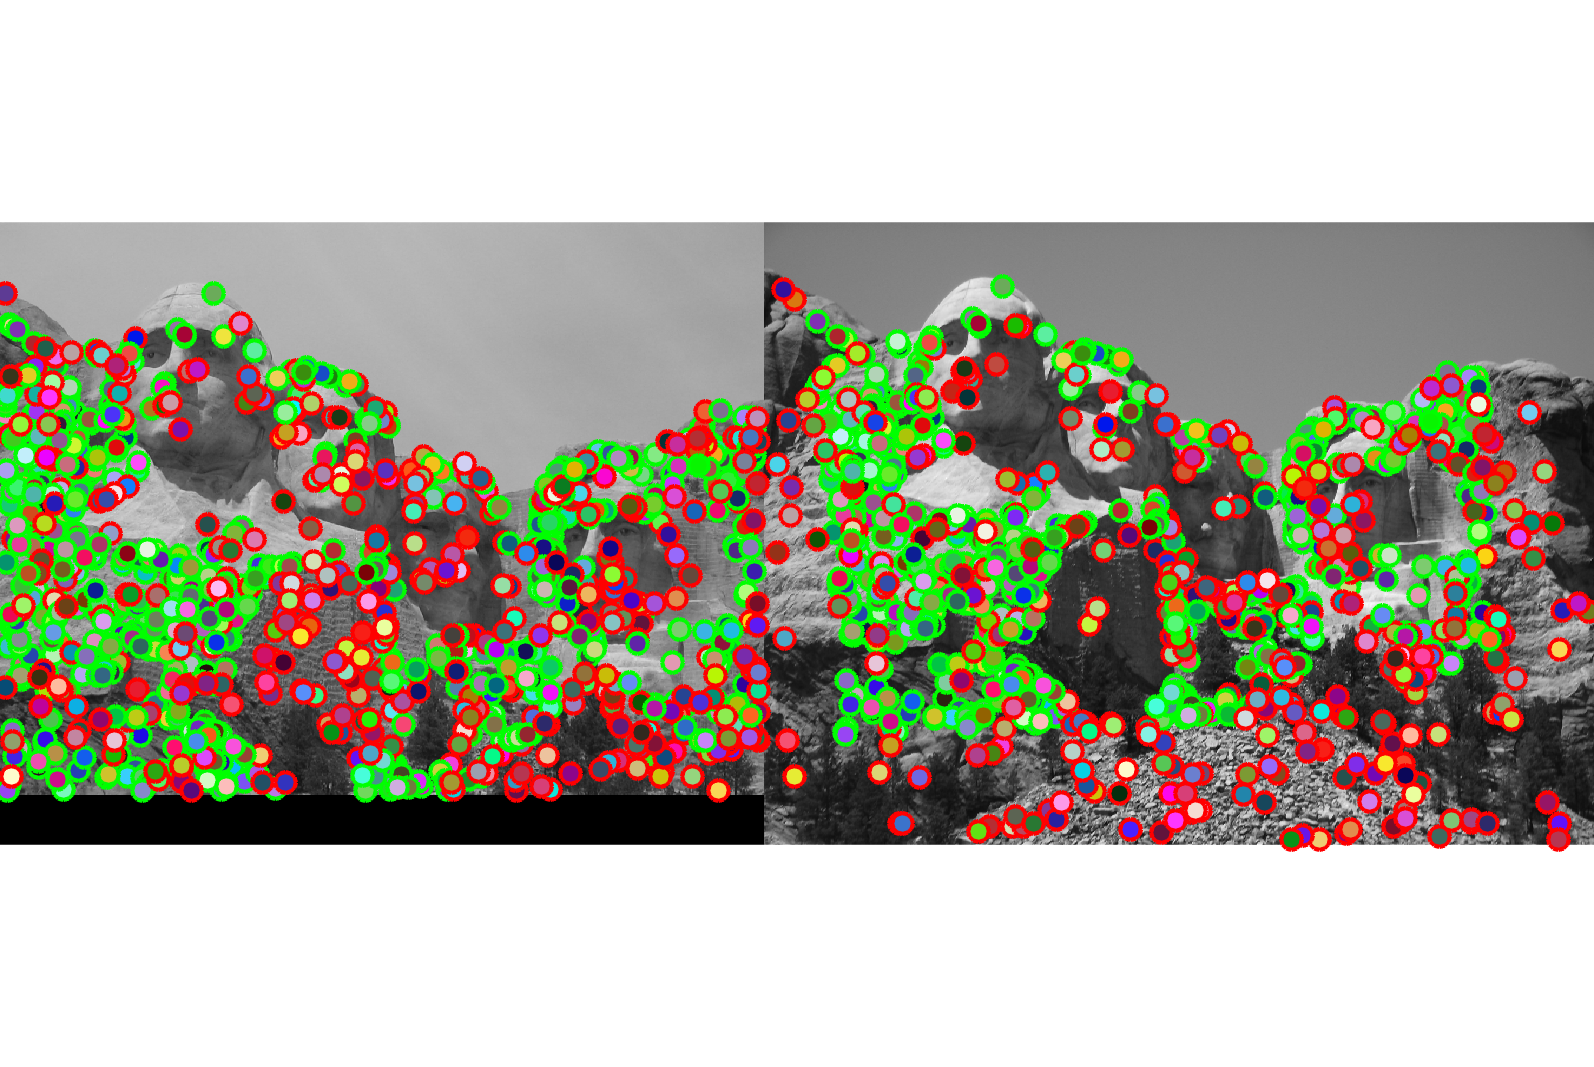
\includegraphics[width=12cm]{../code/eval_MR.png}
    \caption{Result of Mountain Rushmore}
    \label{fig:Mountain Rushmore}
\end{figure}

\begin{figure}[h]
    \centering
    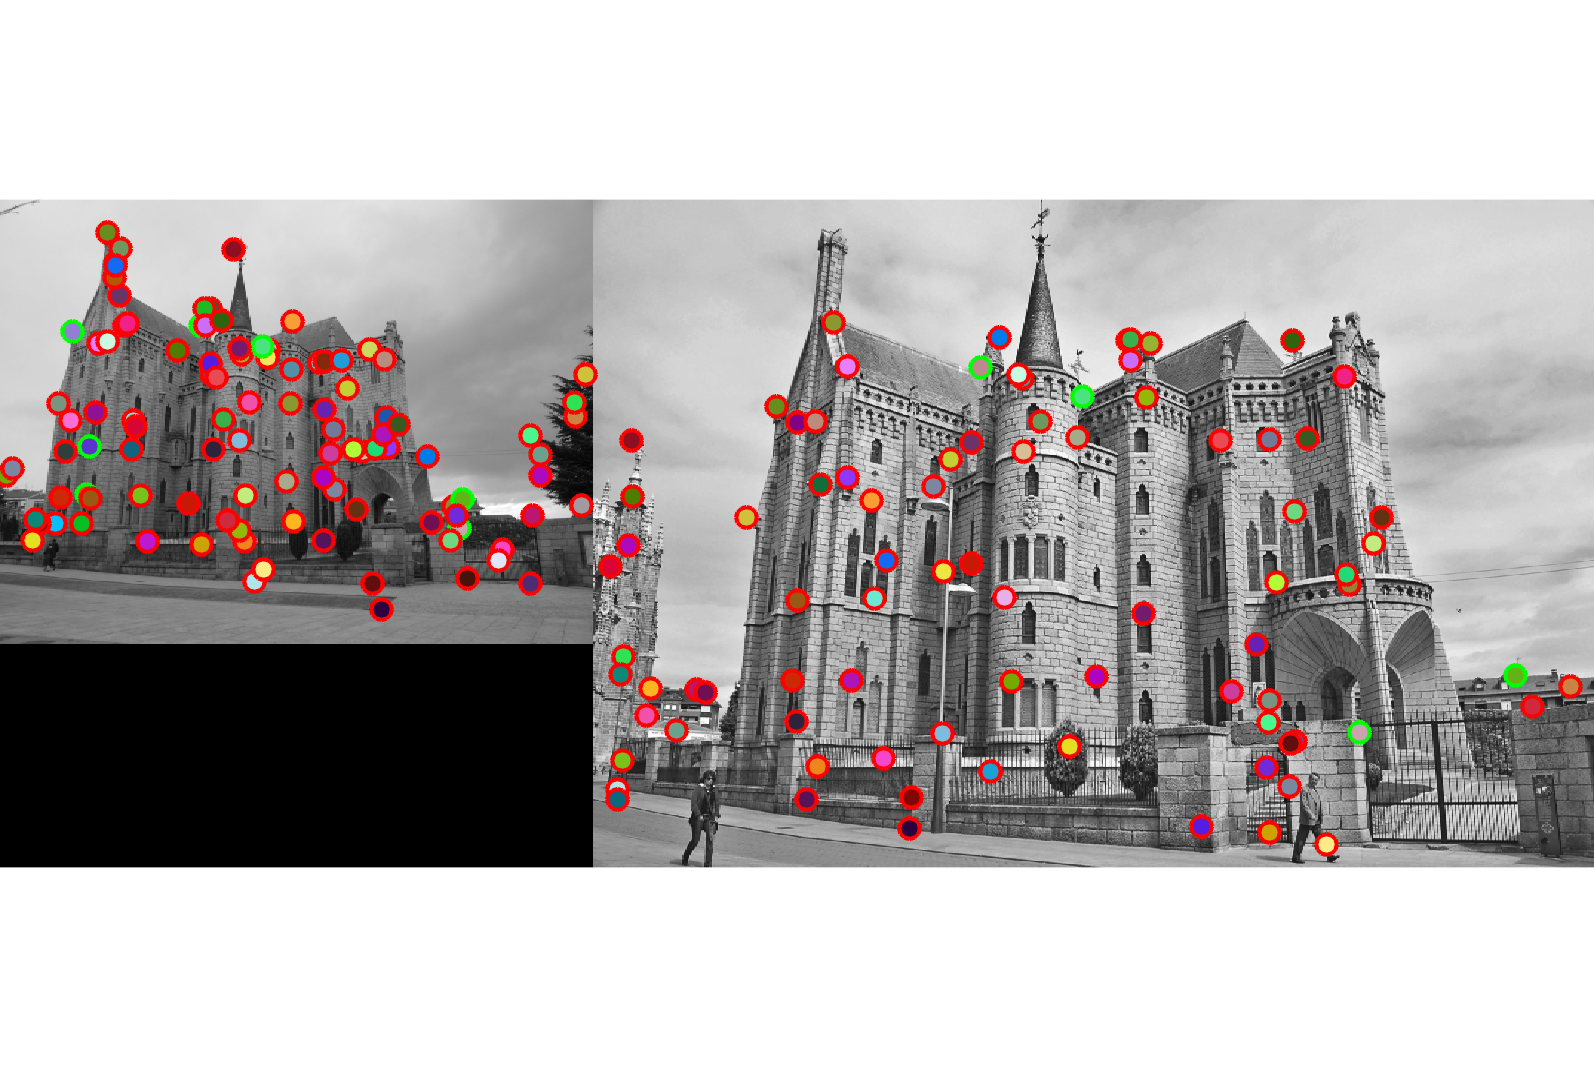
\includegraphics[width=12cm]{../code/eval_EG.png}
    \caption{Result of Gaudi's Episcopal Palace}
    \label{fig:Gaudi's Episcopal Palace}
\end{figure}

\end{document}